\documentclass[../psets.tex]{subfiles}

\pagestyle{main}
\renewcommand{\leftmark}{Homework 5}

\begin{document}




\begin{enumerate}
    \setenumerate[2]{label={\alph*)}}
    \item \marginnote{5/21:}Answer the following questions.
    \begin{enumerate}
        \item Draw a mechanism for the Monsanto acetic acid process.
        \begin{proof}[Answer]
            ${\color{white}hi}$
            \begin{center}
                \begin{tikzpicture}
                    \node (1) at (90:3) {
                        \chemleft{[}
                            \chemfig{Rh(-[1]I)(-[3]OC)(-[5]OC)(-[7]I)}
                        \chemright{]^-}
                    };
                    \node (2) at ([xshift=4mm]-30:3) {
                        \chemleft{[}
                            \chemfig{Rh(-I)(>:[1]I)(-[2]Me)(-[4]OC)(<[5]OC)(-[6]I)}
                        \chemright{]^-}
                    }
                        ([xshift=1mm,yshift=2mm]2.north) edge [blx,semithick,stealth-,bend right=30] ([yshift=-3mm]1.east)
                    ;
                    \node (3) at ([xshift=-8mm]-150:3) {
                        \chemleft{[}
                            \chemfig{Rh(-I)(>:[1]I)(-[2]CO)(-[4](=[:120]O)-[:-120])(<[5]OC)(-[6]I)}
                        \chemright{]^-}
                    }
                        edge [blx,semithick,stealth-,bend right=32] node[black,below]{\small\ce{CO}} (2)
                        ([xshift=1mm,yshift=2mm]3.north)edge [blx,semithick,-stealth,bend left=30] ([yshift=-3mm]1.west)
                    ;
            
                    \node (4) at (135:5) {\chemfig{-[:30](=[2]O)-[:-30]I}}
                        edge [blx,semithick,stealth-,out=-90,in=80] (170:3.28)
                    ;
                    \node (5) at (90:5) {\ce{HI}}
                        edge [blx,semithick,stealth-,bend right=20] ([xshift=4.5mm,yshift=4.5mm]4.center)
                    ;
                    \node (6) at (45:5) {\ce{MeI}}
                        edge [blx,semithick,stealth-,bend right=20] (5)
                        edge [blx,semithick,out=-90,in=100] (10:3.123)
                    ;
            
                    \node (7) at (-4.5,5) {\ce{H2O}};
                    \node (8) at (-1,7) {\chemfig{-[:30](=[2]O)-[:-30]OH}}
                        edge [blx,semithick,stealth-,bend left=50,looseness=1.33] (7)
                    ;
                    \node (9) at (1,6.3) {\ce{MeOH}};
                    \node (10) at (4.5,5) {\ce{H2O}}
                        edge [blx,semithick,stealth-,bend left=50,looseness=1.23] (9)
                    ;
                \end{tikzpicture}
            \end{center}
        \end{proof}
        \item Explain how this mechanism differs for BP's Cativa process.
        \begin{proof}[Answer]
            The most obvious difference is that although the catalysts are similar, the Cativa process uses an iridium center instead of a rhodium one. Additionally, whereas the catalyst from the Monsanto process is purely anionic, the catalyst of the Cativa process has a proton as a counterion. This is notably important when hydroiodic acid is removed from an intermediate. Furthermore, there are a couple alternate pathways and off-cycles to be aware of with the Cativa process. Most notably, the intermediate \ce{Ir(CO)2I2Ac} can be captured and transformed into \ce{Ir(CO)3I2Ac} or \ce{[Ir(CO)2I3Ac]^-H+}. Note that the latter off-cycle product can be generated slowly from the intermediate three steps earlier in the cycle, i.e., \ce{[Ir(CO)2I3Me]^-H+}. Beyond these differences, it is worth noting that the final product (\ce{AcOH}) is pulled directly off of the catalyst by \ce{H2O}, as opposed to through a reductively eliminated \ce{AcI} species. Lastly, the cycle for regenerating \ce{MeI} from \ce{HI} is more complicated in the Cativa process; indeed, while the Monsanto process only uses \ce{MeOH} in one step with \ce{H2O} as a byproduct, the Cativa process uses \ce{MeOAc}, \ce{AcOH}, \ce{MeOH}, and \ce{H2O} in a two-step cycle.
        \end{proof}
    \end{enumerate}
    \item Consider both early and late metal olefin polymerization processes. What is the resting state of the catalyst in each case and why? Predict whether early or late metals should favor linear or branched polyethylene and show a mechanism that explains this.
    \begin{proof}[Answer]
        ${\color{white}hi}$
        \begin{center}
            \schemestart
                \chemfig{M-[:30]-[:-30]-[:30]pl}
                \arrow{<=>}
                \chemfig[]{M(-[7]H)(-[1]\phantom{i}-[::90,0.4,,,white]=_[::180]-[::60]pl)}
            \schemestop
        \end{center}
        Early metal resting state: Metal alkyl intermediate. This is because early metals are terrible backbonders (not enough $d$ electrons) and thus do not form olefin adducts easily. Hence, insertion of an olefin is very fast and a bound olefin is almost never observed in these systems. This favors linear polyethylene because inhibition of olefin adducts precludes chain walking.\par
        Late metal resting state: Metal-olefin adduct. This is because late metals can backbond and will more readily form an olefin adduct. This favors branched polyethylene because metal-olefin adducts are a necessary intermediate to chain walking. Additionally, olefins are more likely to dissociate than alkyls, making chain transfer a more likely possibility.
    \end{proof}
    \item Some catalysts polymerize ethylene to HDPE that contains a few long branches (ca. 1-2 per chain). Explain how the long branches might form. What distribution of branch lengths do you expect for your mechanism?
    \begin{center}
        \schemestart
            \chemfig{=[1]}
            \arrow{->[\small cat]}
            \chemfig[angle increment=30,atom sep=1em]{
                \cdots-[:-15,0.6,,,white]-[1]-[-1]-[1]-[-1]-[1]-[-1]-[1]-[-1]
                (-[-3]-[-1]-[-3]-[-1]-[1]-[-1]-[1]-[-1]-[1]-[-1]-[1]-[-1]-[1]-[:-15,0.6,,,white]\cdots)
                -[1]-[-1]-[1]-[-1]-[1]-[-1]-[1]-[-1]-[1]-[-1]-[1]-[-1]-[1]-[-1]-[:15,0.6,,,white]\cdots
            }
        \schemestop
    \end{center}
    \begin{proof}[Answer]
        The long branches most likely form through chain transfer. If we use early metal catalysts that do not chain walk or dissociate olefins very easily, then we can expect to build only a few very long chains in solution before the inevitable termination step. Once a chain has terminated though, since it has a terminal olefin, there's no reason that a catalyst currently working on another chain couldn't pull in the previously terminated chain at the olefin instead of just another ethylene and then continue on. Indeed something like this would lead to a polymer with only a few very long branches.
    \end{proof}
    \item Provide a concise explanation of the stereocontrol mechanism for the formation of isotactic and syndiotactic polypropylenes by metallocene catalysts of appropriate symmetry. Provide clear drawings to support your discussion.
    \begin{proof}[Answer]
        ${\color{white}hi}$
        \begin{figure}[H]
            \centering
            \begin{subfigure}[b]{0.3\linewidth}
                \centering
                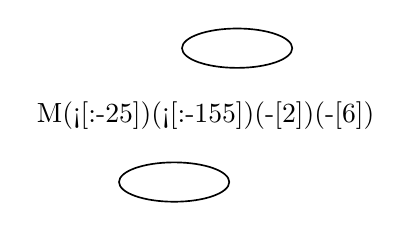
\begin{tikzpicture}
                    \node {\chemfig{M(<[:-25]\coordsite)(<[:-155]\coordsite)(-[2])(-[6])}};
        
                    \filldraw [fill=white,semithick] (0.4,0.85) ellipse (7mm and 2.5mm);
                    \draw [semithick] (-0.4,-0.85) ellipse (7mm and 2.5mm);
                \end{tikzpicture}
                \caption{$C_2$ symmetry.}
                \label{fig:catalysts-polypropylenea}
            \end{subfigure}
            \begin{subfigure}[b]{0.3\linewidth}
                \centering
                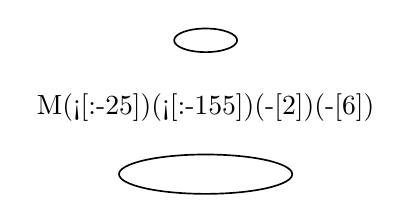
\begin{tikzpicture}
                    \node {\chemfig{M(<[:-25]\coordsite)(<[:-155]\coordsite)(-[2])(-[6])}};
        
                    \filldraw [fill=white,semithick] (0,0.85) ellipse (4mm and 1.5mm);
                    \draw [semithick] (0,-0.85) ellipse (1.1cm and 2.5mm);
                \end{tikzpicture}
                \caption{$C_s$ symmetry.}
                \label{fig:catalysts-polypropyleneb}
            \end{subfigure}
            \caption{Polypropylene-type catalysts.}
            \label{fig:catalysts-polypropylene}
        \end{figure}
        Metallocene catalysts of $C_2$ symmetry will generate isotactic polypropylene. This is because propylene bonds with the same pro-chiral face to each coordination site on Figure \ref{fig:catalysts-polypropylenea} (for the left coordination site, sterics force the methyl group to point upward, and vice versa for the right coordination site). As such, when the chain transfers during a growth step, the methyl group always aligns the same way (always R or always S, depending on whether the pro-R or pro-S face bonds to the catalyst).\par
        On the other hand, metallocene catalysts of $C_s$ symmetry will generate syndiotactic polypropylene. This is because propylene bonds with different pro-chiral faces to each coordination site on Figure \ref{fig:catalysts-polypropyleneb} (at both coordination sites, sterics force the methyl group to point upward). As such, when the chain transfers during a growth step, the methyl group always aligns opposite to the way it aligned last time.
    \end{proof}
    \item Variants of the Wacker oxidation reaction have been developed for the synthesis of fine chemicals and pharmaceuticals. Provide a balanced equation and mechanism for the following intramolecular aza-Wacker cyclization reaction.
    \begin{center}
        \schemestart
            \chemfig{*6(-=(-=^[:30]-[:-30]Me)-(-(=[2]O)-[:-30]NHPh)=-=)}
            \arrow{->[
                \small
                \begin{tabular}{l}
                    \ce{(MeCN)2PdCl2} ($\SI{10}{mol.\%}$)\\
                    \ce{CuCl2} ($\SI{10}{mol.\%}$)\\
                    \ce{NEt3} ($\SI{20}{mol.\%}$)
                \end{tabular}
            ][
                \small
                \begin{tabular}{l}
                    \ce{MeOH} (solvent)\\
                    \ce{O2}\\
                    \textcolor{white}{\ce{(MeCN)2PdCl2} ($\SI{10}{mol.\%}$)}
                \end{tabular}
            ]}[,2.8]
            \chemfig{*6(-=*6(-=(-Me)-NPh-(=O)-)-=-=)}
        \schemestop
    \end{center}
    \begin{proof}[Answer]
        Balanced equation:
        \begin{center}
            \schemestart
                \chemfig{*6(-=(-=^[:30]-[:-30]Me)-(-(=[2]O)-[:-30]NHPh)=-=)}
                \arrow{0}[,0]\+
                \chemfig{\dfrac{1}{2}\, O_2}
                \arrow{->[\small\ce{PdCl2} (cat)][\small\ce{CuCl2} (cat)]}[,1.6]
                \chemfig{*6(-=*6(-=(-Me)-NPh-(=O)-)-=-=)}
                \arrow{0}[,0]\+
                \chemfig{H_2O}
            \schemestop
        \end{center}
        Mechanism:
        \begin{figure}[H]
            \centering
            \setcharge{extra sep=2.5pt}
            \schemestart
                \chemfig{Pd(-[1]NCMe)(-[3]MeCN)(-[5]Cl)(-[7]Cl)}
                \arrow{<=>[*{0}\small\ce{2MeOH}][*{0}\small\ce{2MeCN}]}[-90]
                \chemfig{Pd(-[1]O(-Me)(-[2]H))(-[3]O(-[2]H)(-[4]Me))(-[5]Cl)(-[7]Cl)}
                \arrow{-U>[\footnotesize\chemfig[atom sep=1.3em]{*6(-=(-=^[:30]-[:-30]Me)-(-(=[2]O)-[:-30]NHPh)=-=)}][\footnotesize\ce{MeOH}]}[,1.8]
                \chemfig{*6(-=(-=_[@{Ca1}:30]@{Ca2}(-[::180,0.4,,,opacity=0]\phantom{i}-[::90,1.2]@{Pda}Pd(-[@{Clbond,0.3}:30]@{Cla}Cl)(-[:-60]Cl)(-[:-150]O(-[4]Me)(-[6]H)))-[:-30])-(-(=[2]O)-[:-30]@{Na}\charge{-90=\:}{N}(-[0]Ph)(-[@{Hbond,0.7}2]@{Ha}H))=-=)}
                \arrow{->[\small\chemfig{Me@{Os}\charge{90=\:}{O}H}, \chemfig{@{Ns}\charge{90=\:}{N}Et_3}][\small\ce{-[HNEt3]Cl}]}[,1.7]
                \chemfig{*6(-=*6(-(-Pd(-[0]O(-[1]H)(-[7]Me))(-[4]O(-[3]H)(-[5]Me))(-[6]Cl))-(-)-NPh-(=O)-)-=-=)}
                \arrow{-U>[][*{0}\small\ce{MeOH}][][][90]}[-90,1.5]
                \chemfig{*6(-=*6(-=_(-[::180,0.4,,,opacity=0]\phantom{i}-[::90,1.2]Pd(-[:30]H)(-[:-60]Cl)(-[:-150]O(-[4]Me)(-[6]H)))(-)-NPh-(=O)-)-=-=)}
                \arrow{-U>[\small\ce{MeOH}][\footnotesize\chemfig[atom sep=1.3em]{*6(-=*6(-=(-Me)-NPh-(=O)-)-=-=)}][][][80]}[180,2.1]
                \chemfig{Pd(-[1]H)(-[3]O(-[2]Me)(-[4]H))(-[5]O(-[4]H)(-[6]Me))(-[7]Cl)}
                \arrow{-U>[\small\ce{2MeOH}][\small\ce{HCl}]}[180,2.1]
                \chemfig{Pd(-[1]O(-Me)(-[2]H))(-[3]O(-[2]H)(-[4]Me))(-[5]O(-[4]Me)(-[6]H))(-[7]O(-[6]H)(-[0]Me))}
                \arrow{-U>[][*{0}\small\ce{2MeOH}]}[90,2.3]
            \schemestop
            \chemmove{
                \draw [blx,semithick,shorten <=5pt,shorten >=1pt] (Ns)     to[out=90,in=30] (Ha);
                \draw [blx,semithick,shorten <=2pt,shorten >=1pt] (Hbond)  to[bend left=60,looseness=1.3] (Na);
                \draw [blx,semithick,shorten <=5pt,shorten >=1pt] (Na)     to[out=-90,in=60] (Ca2);
                \draw [blx,semithick,shorten <=7pt,shorten >=1pt] (Ca1)    to[bend right=45,looseness=1.3] (Pda);
                \draw [blx,semithick,shorten <=2pt,shorten >=1pt] (Clbond) to[bend left=60,looseness=1.3] (Cla);
                \draw [blx,semithick,shorten <=5pt,shorten >=1pt] (Os.north)     to[out=120,in=-15,looseness=1.5] (Pda);
            }
            \begin{tikzpicture}[overlay,yshift=-6mm]
                \draw [-stealth] (-5.37,6.3) node[right]{\small\ce{2CuCl2}} arc (260:100:1cm) node[right]{\small\ce{2CuCl}};
                \draw [stealth-] (-4.1,6.3) to[bend right=45] ++(0,2);
                \draw [stealth-] (-3.26,6.3) node[right]{\small\ce{H2O}} to[bend left=45] ++(0,2) node[right,align=left]{\small\ce{\frac{1}{2}O2}\\\small\ce{2HCl}};
            \end{tikzpicture}
        \end{figure}
    \end{proof}
    \item Wilkinson's catalyst catalyzes the hydrosilylation of $\alpha$-olefins, as shown below. Two isomers of the product (\textbf{1}, \textbf{2}) are usually observed and vinylsilanes \textbf{3} are sometimes formed as byproducts. Provide a mechanism for the reaction and the formation of \textbf{1}-\textbf{3}.
    \begin{center}
        \setchemfig{angle increment=30}
        \chemnameinit{\chemfig{R'_3Si-[1](-[3,5]R)=[-1]}}
        \schemestart
            \chemfig{R-[1]=_[-1]}
            \arrow{0}[,0]\+{1em,,0.1em}
            \chemfig{R'_3SiH}
            \arrow{->[\small cat \ce{Rh(PPh3)3Cl}]}[,2]
            \chemname{\chemfig{R-[1]-[-1]-[1]SiR'_3}}{\textbf{1}}
            \+{,,1em}
            \chemname{\chemfig{R-[1](-[3]SiR'_3)-[-1]}}{\textbf{2}}
            \+
            \chemname{\chemfig{R'_3Si-[1](-[3]R)=[-1]}}{\textbf{3}}
        \schemestop
    \end{center}
    \begin{proof}[Answer]
        Product \textbf{1}:
        \begin{center}
            \schemestart
                \chemfig{Rh(-Cl)(-[2]PPh_3)(-[4]Ph_3P)(-[6]PPh_3)}
                \arrow{<=>[][\small\ce{PPh3}]}
                \chemfig{Rh(-Cl)(-[3]Ph_3P)(-[5]Ph_3P)}
                \arrow{->[\small\ce{HSiR$'$3}]}[,1.6]
                \chemfig{Rh(-Cl)(-[2]H)(>:[:160]Ph_3P)(<[:-150]Ph_3P)(-[6]SiR'_3)}
                \arrow{->[*{0}\small\chemfig{=_[:30]-[:-30]R}]}[-90]
                \chemfig{Rh(-\phantom{i}-[6,0.4,,,white]=^[2]-[:30]R)(>:[1]Cl)(-[2]H)(-[4]Ph_3P)(<[5]Ph_3P)(-[6]SiR'_3)}
                \arrow[180]
                \chemfig{Rh(-[:30]-[:-30]-[:30]R)(-[2]Cl)(>:[:160]Ph_3P)(<[:-150]Ph_3P)(-[6]SiR'_3)}
                \arrow{-U>[][*{0.10}\small\chemfig{R-[:30]-[:-30]-[:30]SiR'_3}][][][135]}[90]
            \schemestop
        \end{center}
        Product \textbf{2}:
        \begin{center}
            \schemestart
                \chemfig{Rh(-Cl)(-[2]PPh_3)(-[4]Ph_3P)(-[6]PPh_3)}
                \arrow{<=>[][\small\ce{PPh3}]}
                \chemfig{Rh(-Cl)(-[3]Ph_3P)(-[5]Ph_3P)}
                \arrow{->[\small\ce{HSiR$'$3}]}[,1.3]
                \chemfig{Rh(-Cl)(-[2]H)(>:[:160]Ph_3P)(<[:-150]Ph_3P)(-[6]SiR'_3)}
                \arrow{->[*{0}\small\chemfig{=_[:30]-[:-30]R}]}[-90]
                \chemfig{Rh(-\phantom{i}-[6,0.4,,,white]=^[2]-[:30]R)(>:[1]Cl)(-[2]H)(-[4]Ph_3P)(<[5]Ph_3P)(-[6]SiR'_3)}
                \arrow[180]
                \chemfig{Rh(-(-[:60]R)(-[:-60]))(-[2]Cl)(>:[:160]Ph_3P)(<[:-150]Ph_3P)(-[6]SiR'_3)}
                \arrow{-U>[][*{0.30}\small\chemfig{R-[:30](-[2]SiR'_3)-[:-30]}][][][135]}[90]
            \schemestop
        \end{center}
        Product \textbf{3}:
        \begin{center}
            \schemestart
                \chemfig{Rh(-Cl)(-[2]PPh_3)(-[4]Ph_3P)(-[6]PPh_3)}
                \arrow{<=>[][\small\ce{PPh3}]}
                \chemfig{Rh(-Cl)(-[3]Ph_3P)(-[5]Ph_3P)}
                \arrow{->[\small\ce{HSiR$'$3}]}[,1.7]
                \chemfig{Rh(-Cl)(-[2]H)(>:[:160]Ph_3P)(<[:-150]Ph_3P)(-[6]SiR'_3)}
                \arrow{->[*{0}\small\chemfig{=_[:30]-[:-30]R}]}[-90]
                \chemfig{Rh(-\phantom{i}-[6,0.4,,,white]=^[2]-[:30]R)(>:[1]Cl)(-[2]H)(-[4]Ph_3P)(<[5]Ph_3P)(-[6]SiR'_3)}
                \arrow[-90]
                \chemfig{Rh(-[:30]-[:-30](-[6]SiR'_3)-[:30]R)(-[2]H)(>:[:160]Ph_3P)(<[:-150]Ph_3P)(-[6]Cl)}
                \arrow[180]
                \chemfig{Rh(-[,1.3]\phantom{i}-[2,0.4,,,white]=[6](-[:-150]R)(-[:-30]SiR'_3))(>:[1]H)(-[2]H)(-[4]Ph_3P)(<[5]Ph_3P)(-[6]Cl)}
                \arrow{-U>[][*{0.30}\small\chemfig{R'_3Si-[:30](-[2]R)=[:-30]}][][][135]}[90]
                \chemfig{Rh(-H)(-[2]H)(>:[:160]Ph_3P)(<[:-150]Ph_3P)(-[6]Cl)}
                \arrow{-U>[][*{0}\small\ce{H2}][][][90]}[90,1.1]
            \schemestop
        \end{center}
    \end{proof}
    \item This question is meant to guide you through Prof. Jack Halpern's paper studying the enantioselective hydrogenation of methyl-(Z)-$\alpha$-acetamidocinnamate (mac) mediated by \ce{[Ru({dipamp})(MeOH)2]+} \parencite{bib:HalpernHydrogenation}. These questions will focus on the introduction, results, and discussion (not the experimental section).
    \begin{enumerate}
        \item Figure 1 depicts a previously published achiral hydrogenation catalyst. Draw the cycle in Figure 1 and label the mechanism for each step. When drawing arrows between intermediates, indicate whether the step is reversible and, if so, which intermediate is favored. Label the rate determining step at room temperature (RT) and at $\SI{-40}{\celsius}$.
        \begin{proof}[Answer]
            ${\color{white}hi}$
            \begin{center}
                \setlength{\tabcolsep}{0pt}
                \schemestart
                    \chemleft{[}
                        \chemfig{Rh(-[3]\chemabove{P}{Ph_2}-[:-150]?)(-[5]\chembelow{P}{Ph_2}-[:150]?)(-[7]S)(-[1]S)}
                    \chemright{]^+}
                    \arrow{<->>[\footnotesize\chemfig[atom sep=1.3em]{-[2](=[:150]O)-[:30]NH-[2](=_[:150]-[2]Ph)-[:30](=[2]O)-[:-30]O-[:30]}][\scriptsize coordination]}[,1.9]
                    \chemleft{[}
                        \chemfig{Rh?[Rh](-[3]\chemabove{P}{Ph_2}-[:-150]?[P])(-[5]\chembelow{P}{Ph_2}-[:150]?[P])(-[:-35]O=[:0](-[::-60])-[::60]NH-[::60](=^[::60](-[::180,0.4,,,opacity=0]\phantom{i}?[Rh])-[::-60]Ph)-[::-60](=[::60]O)-[::-60]O-[::60])}
                    \chemright{]^+}
                    \arrow{->[*{0}\small\ce{H2}][*{0}\scriptsize\begin{tabular}{r} oxidative\\addition\vspace{1em}\\RDS (RT) \end{tabular}]}[-90,1.3]
                    \chemleft{[}
                        \chemfig{Rh?[Rh](-[4]\chemabove{P}{Ph_2}-[:-150]?[P])(<[5]\chembelow{P}{Ph_2}-[:-165]?[P])(-[6]O=[:0](-[::-60])-[::50]NH-[::50](=^[::50](-[::180,0.4,,,opacity=0]\phantom{i}?[Rh,6])-[::-60]Ph)-[::-70](=[::60]O)-[::-60]O-[::60])(-H)(-[2]H)}
                    \chemright{]^+}
                    \arrow(--a){->[\small\ce{S}][\scriptsize\begin{tabular}{c} migratory\\insertion \end{tabular}]}[180,1.3]
                    \chemleft{[}
                        \chemfig{Rh?[Rh](-[4]\chemabove{P}{Ph_2}-[:-150]?[P])(<[5]\chembelow{P}{Ph_2}-[:-165]?[P])(-O=[:20](-[::-60])-[::70,0.8]NH-[::70]?[Rh,6](-[::40]-[::-60]Ph)-[::-60,0.6](=[::60,0.8]O)-[::-60,0.7]O-[::60,0.6])(-[6]S)(-[2]H)}
                    \chemright{]^+}
                    \arrow{-U>[*{0}\small\ce{S}][*{0.30}\footnotesize\hbox{\chemfig[atom sep=1.3em]{-[2](=[:150]O)-[:30]NH-[2](-[:150]-[2]Ph)-[:30](=[2]O)-[:-30]O-[:30]}}][][][90]}[90,1.6]
                    \arrow(@a--){0[][*{0}\scriptsize\begin{tabular}{l} reductive\\elimination\vspace{1em}\\RDS ($\SI{-40}{\celsius}$) \end{tabular}]}[90,1.6]
                \schemestop
            \end{center}
        \end{proof}
        \item Figure 2 depicts two possible catalytic cycles for the asymmetric catalyst \ce{[Ru({dipamp})(MeOH)2]+}. In this scheme, why is one labeled the "major manifold" and the other the "minor manifold?" Why does the minor manifold lead to the major product? Depict the differences in energy for each pathway with a reaction coordinate diagram (we used these to talk about catalysis on May 1) and indicate the resting state of the catalyst.
        \begin{proof}[Answer]
            ${\color{white}hi}$
            \begin{figure}[H]
                \centering
                \begin{tikzpicture}[
                    out=0,in=180,
                    every node/.style={black,fill=white,inner sep=1.5pt}
                ]
                    \draw [rex,dashed,thick] (5,-1) -- ++(0,5) node[left=5mm]{Major} node[right=5mm]{Minor};
            
                    \draw [blx,thick]
                           (0,0) node[below]{\footnotesize Product}
                        to (2,3)
                        to (3.5,1) node[below]{\footnotesize\ce{[Rh(dipamp)(mac)]+}}
                        to (4.5,2.5)
                        to (5,2) node[below]{\footnotesize mac}
                        to (5.7,2.8)
                        to (6,2.6) node[anchor=167]{\footnotesize\ce{[Rh(dipamp)(mac)]+}}
                        to (6.7,2.9)
                        to (8.5,0) node[below]{\footnotesize Product}
                    ;
                \end{tikzpicture}
                \caption{Reaction coordinate diagram.}
                \label{fig:reactionCoordinate}
            \end{figure}
            This whole paper centers around the chirality of the \ce{[Rh(dipamp)(mac)]+} adduct and, thus, the stereochemistry of the product. Of course, sometimes diastereomers (such as the two possible \ce{[Rh(dipamp)(mac)]+} adducts) can have slightly different properties. As such, the major manifold follows the catalysis using the more thermodynamically stable "major" \ce{[Rh(dipamp)(mac)]+} adduct (probably called major since its thermodynamic stability means that there is relatively more of it in solution), and likewise for the minor manifold.\par
            It is exactly this variability in stability that causes the minor manifold to yield the major product and vice versa; indeed, since the minor adduct is less thermodynamically stable and much more reactive with \ce{H2}, it reacts faster and creates more of its product.\par
            The reaction coordinate diagram shows that the energy of the minor adduct is higher and the energy of the major adduct is lower, affecting their relative concentrations in solution as discussed. However, this also means that the remainder of the steps are harder, since we've overstabilized the intermediate and it's already less reactive with \ce{H2}.
        \end{proof}
        \item The substrate mac can form two different isomers by associating with the metal catalyst. These complexes are termed $2^\text{min}$ and $2^\text{maj}$. Provide an example of a spectroscopic technique where the two complexes can be differentiated and an example where they appear identical.
        \begin{proof}[Answer]
            As stereoisomers, NMR can differentiate between them, but they would appear identical to mass spectroscopy.
        \end{proof}
        \item To gain insight on the mechanism of hydrogenation and the origin of enantioselectivity, the influence of varying \ce{H2} pressures on the rates of catalysis is explored. Under what conditions is the oxidative addition the rate determining step, and under what conditions is isomerization between $2^\text{maj}$ and $2^\text{min}$ the rate determining process? These studies are shown in Figure 6; explain the changes in the rate of formation of the S-product observed upon changing the pressure of \ce{H2}.
        \begin{proof}[Answer]
            Oxidative addition is the RDS at sufficiently low pressures of \ce{H2}, since there it finally becomes slower than reductive elimination. Isomerization between $2^\text{maj}$ and $2^\text{min}$ is the RDS at sufficiently high pressures of \ce{H2}, since in the limit of infinitely high \ce{H2} pressure, oxidative addition finally becomes faster than isomerization.\par
            As \ce{[H2]} increases, the reaction rate increases. As it does, since the S-product is the major product, as formed by the less thermodynamically stable, more reactive minor adduct, the differences in how much more of it is formed will be exaggerated.
        \end{proof}
        \item What does it mean for the selectivity of a reaction to be "product controlled?"
        \begin{proof}[Answer]
            In the sense of the Hammond postulate, it means that the stability of the products determines the activation energy of the reaction (esp. the energy of the transition state). With respect to the catalytic method under study here, it is applied to the fact that the greater stability of the minor \emph{dihydride} adduct (see Figure 9 in \textcite{bib:HalpernHydrogenation}) causes the process of conversion to it to be less energy intensive than the analogous process for the major \emph{dihydride} adduct.
        \end{proof}
    \end{enumerate}
\end{enumerate}




\end{document}